%%%%%%%%%%%%%%%%%%%% author.tex %%%%%%%%%%%%%%%%%%%%%%%%%%%%%%%%%%%
%
% sample root file for your "contribution" to a contributed volume
%
% Use this file as a template for your own input.
%
%%%%%%%%%%%%%%%% Springer %%%%%%%%%%%%%%%%%%%%%%%%%%%%%%%%%%


% RECOMMENDED %%%%%%%%%%%%%%%%%%%%%%%%%%%%%%%%%%%%%%%%%%%%%%%%%%%
\documentclass[graybox]{svmult}

% choose options for [] as required from the list
% in the Reference Guide

\usepackage{mathptmx}       % selects Times Roman as basic font
\usepackage{helvet}         % selects Helvetica as sans-serif font
\usepackage{courier}        % selects Courier as typewriter font
\usepackage{type1cm}        % activate if the above 3 fonts are
                            % not available on your system
%
\usepackage{makeidx}         % allows index generation
\usepackage{graphicx}        % standard LaTeX graphics tool
                             % when including figure files
\usepackage{multicol}        % used for the two-column index
\usepackage[bottom]{footmisc}% places footnotes at page bottom

\usepackage{natbib}
\usepackage{aas_macros}

\usepackage{subfigure}

% see the list of further useful packages
% in the Reference Guide

% Added:

\usepackage{ amssymb }


\makeindex             % used for the subject index
                       % please use the style svind.ist with
                       % your makeindex program

%%%%%%%%%%%%%%%%%%%%%%%%%%%%%%%%%%%%%%%%%%%%%%%%%%%%%%%%%%%%%%%%%%%%%%%%%%%%%%%%%%%%%%%%%

\begin{document}

\title*{Long baseline imaging with LOFAR}
% Use \titlerunning{Short Title} for an abbreviated version of
% your contribution title if the original one is too long
\author{Javier Mold\'{o}n and Eskil Varenius}
% Use \authorrunning{Short Title} for an abbreviated version of
\authorrunning{J. Mold\'{o}n and E. Varenius}
% your contribution title if the original one is too long
\institute{Javier Mold\'{o}n \at ASTRON, Postbus 2, 7990 AA Dwingeloo, The Netherlands, \email{moldon@astron.nl}
\and Eskil Varenius \at Onsala Space Observatory, Dept. of Earth and Space Sciences, Chalmers University of Technology, SE-43992 Onsala, Sweden  \email{varenius@chalmers.se}
}
%\and Name of Second Author \at Name, Address of Institute \email{name@email.address}}
%
% Use the package "url.sty" to avoid
% problems with special characters
% used in your e-mail or web address
%
\maketitle

\abstract*{In this chapter we focus on the calibration of International LOFAR,
which includes the long baselines provided by international stations, to produce
high-resolution radio images. The Very Long Baseline Interferometry (VLBI)
techniques are explained, as well as the different steps required to properly
calibrate a long-baseline observation at low frequencies.}

%\abstract{In this chapter we focus on the calibration of International LOFAR,
%which includes the long baselines provided by international stations, to produce
%high-resolution radio images. The Very Long Baseline Interferometry (VLBI)
%techniques are explained, as well as the different steps required to properly
%calibrate a long-baseline observation at low frequencies.}

% Learning Specifics
% In this chapter we focus on the calibration of International LOFAR, which includes
% the long baselines provided by international stations, to produce high-resolution
% radio images. The Very Long Baseline Interferometry (VLBI) techniques are ex-
% plained, as well as the different steps required to properly calibrate a long-baseline
% observation at low frequencies.
% Learning Objectives
% -  To understand the key differences between short- and long-baseline interferome-
% try.
% -  To understand the scales for LOFAR VLBI: resolution and field of view.
% -  To understand the variables relevant for long baseline interferometry: phase, de-
% lay, delay rate.
% -  To understand the impact of baseline separation, ionosphere, and source structure
% on the phase behavior.
% -  To understand how the phase calibration is conducted in VLBI.
% -  To know what calibrators are needed in a typical long baseline observation.
% -  To understand the differences between cm-VLBI and m-VLBI. To understand
% the dispersive delay produced by the ionosphere.
% -  To know how to form a sensitive tied station from the LOFAR core stations.
% -  To understand why circular polarization is useful and how to convert the data.
% -  To know how to combine sub-bands in a measurement set to form a FITS file.
% -  To know how to manage FITS files, convert them, and manipulate them in AIPS.
% -  To know how to conduct a VLBI phase calibration in AIPS.
% -  To know how to inspect phase solutions and to understand their meaning.
% -  To know possible ways to obtain the amplitude calibration for international sta-
% tions.
% -  To know how to produce high-resolution radio images.

\section{Introduction}
\label{sec:introduction}

The prime reason to include the international LOFAR stations in the array is to
obtain very high-resolution images.  Using the longest LOFAR baselines,
subarcsecond imaging is possible with High Band Array (HBA) and the upper part
of the Low Band Array (LBA). Early science results include images of AGN jets,
and of individual supernova remnants in M82 (see Fig. \ref{fig:m82}).  In this
chapter we describe the international LOFAR stations and, in general terms,
some important things to keep in mind when observing, calibrating and imaging
data including \emph{long} baselines, i.e.  baselines to international
stations.  In particular we summarise how techniques from Very Long Baseline
Interferometry (VLBI) can be used to calibrate LOFAR data using the longest
baselines. Some parts of the text are focused on HBA data; calibration and
imaging of long baseline data from the LBA is more challenging and additional
work is still needed to find the best approach. 

\begin{figure}
%\sidecaption[t]
\begin{center}
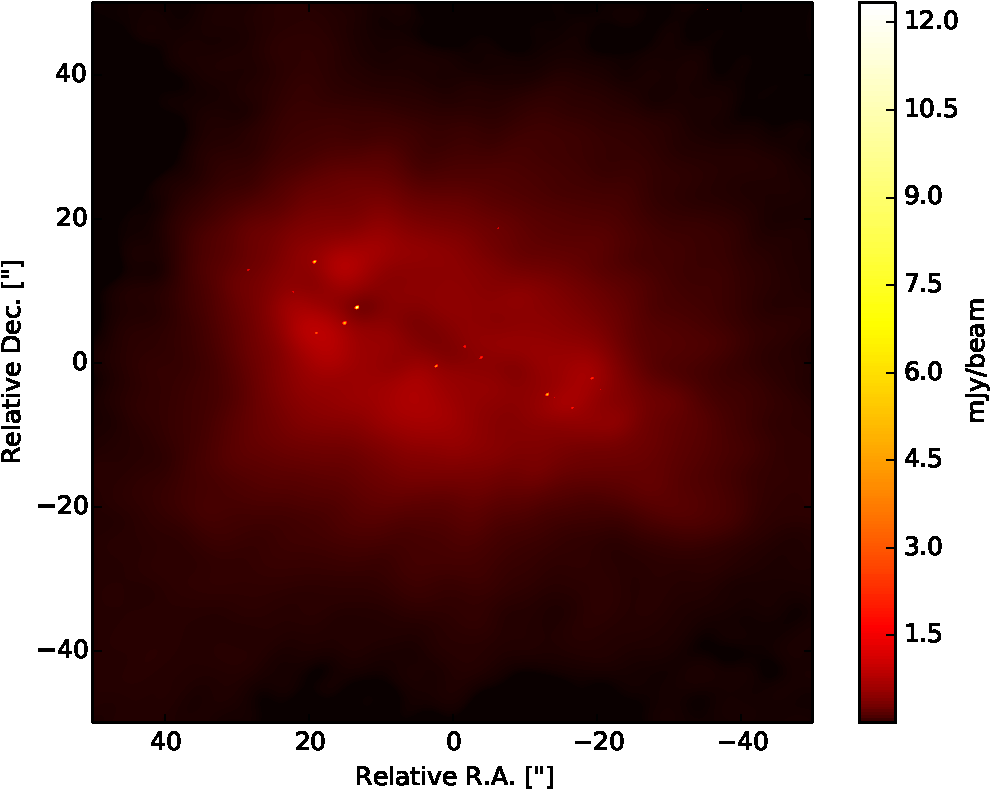
\includegraphics[width=\textwidth]{figures/M82HIGH_FEATHER-crop.pdf}
\caption{Combined high resolution and low resolution image of M82 illustrating
the relative brightness between the compact and extended emission at 154\,MHz.
The synthesized beam size of the International LOFAR image is
$0.36''\times0.23''$ and has an rms noise level of 0.15~mJy/beam. \citep{varenius15}}
\label{fig:m82}
\end{center}
\end{figure}

The outline of this chapter is as follows: in Sect. \ref{sect:intlofar} we
decribe the international LOFAR stations and what to expect in general in
terms of resolution, sensitivity and field of view. In Sect. \ref{sect:calibration}
we describe how to calibrate visibility phases and amplitudes using
data on the longest LOFAR baselines, in particular how to deal
with residual delays and rates. In Sect. \ref{sect:obsstrat} we summarise
the optimal observing strategy for enabling calibration of the international
stations. Finally in Sect. \ref{sect:practical} we discuss a few practical
considerations which may be useful when working with LOFAR data including
international stations.

\section{The international LOFAR stations}
\label{sect:intlofar}
The majority of the LOFAR stations, namely the core and remote stations, are
distributed over an area roughly 180 km in diameter predominantly in the
northeastern Dutch province of Drenthe. Currently, the array also includes 9
international LOFAR stations across Europe that provide maximum baselines up to
1292~km. Three additional stations are under construction in Poland,
extending the maximum baseline to $\sim$2000~km. Fig.~\ref{fig:stations} shows
the distribution of stations already existing or currently under construction.

%Observations with the LOFAR international stations are different from the Dutch
%array observations in that the number of stations providing baselines above
%120~km is scarce, yielding a less dense uv-coverage, that the instrument has a
%reduced field of view (FoV), and that the atmospheric conditions above each
%station are highly uncorrelated, making the phase calibration much more
%delicate. Another (current) difference is that a catalogue of compact sources at
%frequencies below 300~MHz does not exist, and no accurate models of the compact
%structure of flux calibrators is available.

\begin{figure}[t]
%\sidecaption[t]
\begin{center}
\includegraphics[width=\textwidth]{figures/LOFAR_stations_map.jpg}
\caption{LOFAR is composed by 24 core stations and 13 remote stations in the
Netherlands, and 9 international stations (+3 under construction).}
\label{fig:stations}
\end{center}
\end{figure}


\subsection{Sampling of Fourier space}\label{sec:uvcoverage}
The core stations provide maximum baselines of 2.7~km, the remote stations of
120~km, and the international stations of 1300~km.  Table~\ref{tab:baselines}
shows the distances between each pair of international stations, including the
core station CS001 as a reference to the centre of the array.  Since there are
relatively few international stations, the sampling of Fourier space
($uv$-coverage) is less dense for baselines to international stations compared
to core- and remote baselines.  A typical LOFAR $uv$ coverage is shown in
Fig.~\ref{fig:uvcoverage}.  It should be noted that because of the wide
bandwidth offered by LOFAR, Multi-Frequency-Synthesis techniques can be used in
imaging to provide very good $uv$-coverage also at the longest baselines.  

\begin{table}[h]
\centering
\begin{tabular}{ccccccccccc}
\hline
\hline
      & CS001& DE609& DE605& DE601& DE603& DE604& DE602& SE607& UK608& FR606 \\
\hline
 CS001&     0&   224&   226&   266&   396&   419&   581&   594&   602&   700 \\
 DE609&   224&     0&   394&   412&   325&   248&   585&   430&   825&   892 \\
 DE605&   226&   394&     0&    53&   372&   487&   440&   807&   552&   498 \\
 DE601&   266&   412&    53&     0&   344&   476&   390&   833&   590&   490 \\
 DE603&   396&   325&   372&   344&     0&   186&   277&   714&   920&   800 \\
 DE604&   419&   248&   487&   476&   186&     0&   455&   556&  1005&   957 \\
 DE602&   581&   585&   440&   390&   277&   455&     0&   990&   959&   690 \\
 SE607&   594&   430&   807&   833&   714&   556&   990&     0&  1110&  1292 \\
 UK608&   602&   825&   552&   590&   920&  1005&   959&  1110&     0&   495 \\
 FR606&   700&   892&   498&   490&   800&   957&   690&  1292&   495&     0 \\
\hline
\end{tabular}
\caption{Separation in km between the Dutch core and the currently available
international stations.
\label{tab:baselines}}
\end{table}


\begin{figure}[t]
\begin{center}
\includegraphics[width=\textwidth]{figures/uv_cov.png}
\caption{$uv$ coverage for a 4-hr observation of a source at declination
$+48^{\circ}$ with a single subband centred at 140~MHz. Only one visibility every 160 seconds is shown. The rectangles in the last three panels show the area covered by the previous panel. Visibilities corresponding to baselines with international
stations are plotted in red.}
\label{fig:uvcoverage}
\end{center}
\end{figure}

%
%\begin{table}
%\caption{Current international LOFAR stations}             % title of Table
%\label{tab:ilofarstations}      % is used to refer this table in the text
%\centering                          % used for centering table
%\begin{tabular}{l c c} 
%\hline\hline
%Station & Distance to  &  Corresponding resolution  \\
%        & LOFAR core (km) &  at 140 MHz ($^{\prime\prime}$) \\
%\hline
%DE605  & 226  &  2.4  \\
%DE601  & 266  &  2.0  \\
%DE603  & 396  &  1.4  \\
%DE604  & 419  &  1.3  \\
%DE602  & 581  &  0.9  \\
%SE607  & 594  &  0.9  \\
%UK608  & 602  &  0.9  \\
%FR606  & 700  &  0.8  \\
%\hline                                   %inserts single line
%\end{tabular}
%\end{table}

\subsection{Resolution and sensitivity}
In general, the image resolution from interferometric data depends on the
sampling of fourier space and relative weighting applied to the visibilities
when imaging.  A quick estimate can however be obtained using the well known
expression  $\theta \approx \lambda / D$ where $\lambda$ is the wavelength of
the observation, $D$ is the maximum baseline length, and $\theta$ is the angular
resolution in radians.  For international LOFAR baselines we estimate an angular
resolution of about 0.3'' at 150\,MHz.  This is also verified in practice, for
example in the observations of M82 \cite{varenius15}. Estimates for LBA and HBA
can be found in Sect.~\ref{sect:smearing}.

The expected image noise depends on many factors, such as which baselines to
include in the final imaging, but also on the solar activity at the time of
observation.  For subarcsecond imaging it is common to exclude the NL-baselines
and only include data on baselines to international stations.  LOFAR HBA is most
sensitive at frequencies around 150\,MHz \citep[Fig.  22]{vanhaarlem13}.
\cite{varenius15} obtained rms noise levels of 0.3\,mJy/beam at 118\,MHz and
0.15\,mJy/beam at 154\,MHz using 16\,MHz bandwidth and 16 hours of integration,
in reasonable agreement with theoretical estimates (see \cite{varenius15} for a
brief discussion on the expected thermal noise).  Since then, more international
stations have became available and station calibration has been improved. It is
reasonable to assume similar rms noise levels (scaling with bandwidth and
intergration time) can be expected in future observations using international
baselines.

\subsection{Field of view}
%\section{The small field of view approximation}
\label{sec:fov}
The sky area possible to image from any LOFAR observation is limited by factors
such as the station beam, baseline projection effects, and atmospheric
disturbances across the sky. NL-LOFAR observations are often also limited by
very bright interfering sources, such as the \emph{A-team}.  International
baseline imaging is in many aspects simpler than Dutch baseline imaging, because
we can generally ignore interference from other bright sources in the sky.

For a distant potentially interfering source, the interfering contribution to
the target source visibility declines by factors of $u^{-1}$ as a function of
baseline length ($u$)  for both frequency and time decorrelation (also called
\emph{smearing}).  Furthermore, for  most  of the source population resolved on
longer Dutch LOFAR baselines, the intrinsic visibility structure decreases
faster than $u^{-2}$ (a rough approximation based on experience of typical
dependence of visibility amplitude vs baseline length for resolved radio
sources), giving a total decrease of interfering signals with baseline length
scaling as $ u^{-4}$. This means that the effect of interfering signals is a
million times less for baselines of 1000\,km as opposed to 30\,km. This effect
explains why the influence of the brightest sources at LOFAR frequencies, like
Cassiopeia A or Cygnus A, can be ignored at international baseline resolution,
as can most Jansky level sources within the station beam.

For very high-resolution imaging we are often interested in specific objects
covering a small part of the sky. This small field of view regime is where
cm-VLBI usually operates and this regime greatly simplifies imaging. In this
regime, target images are generally smaller than the isoplanatic patch, and
therefore only a single-direction station-dependent correction needs to be
determined.  Likewise, over such small fields, $w$-term effects and station beam
variations can generally be ignored.  This is different from LOFAR
core-resolution imaging, where in order to get noise-limited (rather than
``dynamic range''-limited) images at any given point in a field the whole field
must be imaged using multi-directional calibration techniques.

Whether one can produce useful images using the small-field approximation and
VLBI software depends on the brightness of the target source and, if necessary,
the availability of close sources to use as calibrators similar to what is done
in cm-VLBI.

\subsubsection{Time and frequency smearing}
\label{sect:smearing}
Although smearing helps to simplify calibration by reducing the influence of
bright interfering sources, care has to be taken to not average too much so that
the science targets are affected. In this section we estimate the impact of
smearing on the field of view.

For LOFAR, the standard
\emph{raw} data are delivered from the correlator with resolution 1 second in
time, and 64 channels per subband.  Each subband (using the standard 200\,MHz
clock) is 195\,kHz wide, meaning that the default minimum averaging bandwidth is
3~kHz. This will limit the dynamic range at some distance from the observed
phase centre, similar to the limit imposed by the station beam.  A detailed
description of the averaging losses is beyond the scope of this chapter, we
merely quote the often used results by \cite{taylor99} chapter 18, who derived
two expressions to estimate the average amplitude loss due to averaging in
frequency and time, at some distance from the phase centre.  For frequency
smearing, we can use their expression 18-24 assuming a square bandpass and
circular Gaussian tapering, where the reduction in amplitude at a distance from
the phase centre $r$ can be estimated as
\begin{equation}
\frac{I}{I_0} = \frac{\sqrt{\pi}}{2\sqrt{\ln{2}}}\frac{\theta \nu_c}{r \Delta
\nu}\mathrm{erf}\left(\sqrt{\ln{2}}\frac{r \Delta\nu}{\theta \nu_c}\right)
\label{eqn:freqloss}
\end{equation}
where $\theta$ is the synthesized beam size (FWHM), $\nu_c$ is the central
frequency of the observation, and $\Delta \nu$ is the bandwidth. Note that the
units of $\theta$ and $r$ cancel if they are given in the same unit. Note also
that this expression is in fact independent of central frequency $\nu_c$ since
the synthesised beam also scales with $\nu_c$, only the bandwidth is important.

For time smearing, we may use their formula 18-43, assuming a 12 hour average
over a circular UV-coverage with Gaussian tapering:
\begin{equation}
\frac{I}{I_0} = 1-1.22\times 10^{-9}\left(\frac{r}{\theta}\right)^2\Delta t^2
\label{eqn:timeloss}
\end{equation}
where $\Delta t$ is the averaging time in seconds.

What loss to define as acceptable of course depends on your science, in
particular the brightness of your target, but as a general guide one may
tolerate 5\% loss in amplitude due to averaging. Using the standard LOFAR raw
data values, we have calculated the corresponding circle (diameter, to compare
with station FWHM) for different observing frequencies, see Table \ref{tab:res}.
We have also included estimates for a typical long baseline observation
averaging to 2s and 4ch/subband.

\begin{table}[h]
\centering
\begin{tabular}{rrrr|rr|rr}
\hline\hline
Freq. & $\lambda$ & Int. PSF & Int. station& 5\% loss, 1s& 5\% loss, 64ch/SB & 5\% loss, 2s& 5\% loss, 4ch/SB\\
(MHz) & (m) & FWHM ($''$) & FHWM (deg) & Diam. (deg) & Diam. (deg) & Diam. (deg) & Diam. (deg)\\
\hline
 15 & 19.99 & 2.54&19.39 & 9.02 & 3.30& 4.51 & 0.21\\
 30 & 9.99 & 1.27 & 9.70 & 4.51 & 3.30& 2.26 & 0.21\\
 45 & 6.66 & 0.85 & 6.46 & 3.01 & 3.30& 1.50 & 0.21\\
 60 & 5.00 & 0.63 & 4.85 & 2.26 & 3.30& 1.13 & 0.21\\
 75 & 4.00 & 0.51 & 3.88 & 1.80 & 3.30& 0.90 & 0.21\\
120 & 2.50 & 0.32 & 2.59 & 1.13 & 3.30& 0.56 & 0.21\\
150 & 2.00 & 0.25 & 2.07 & 0.90 & 3.30& 0.45 & 0.21\\
180 & 1.67 & 0.21 & 1.73 & 0.75 & 3.30& 0.38 & 0.21\\
200 & 1.50 & 0.19 & 1.55 & 0.68 & 3.30& 0.34 & 0.21\\
210 & 1.43 & 0.18 & 1.48 & 0.64 & 3.30& 0.32 & 0.21\\
240 & 1.25 & 0.16 & 1.29 & 0.56 & 3.30& 0.28 & 0.21\\

\hline
\end{tabular}
\caption{Station FWHM Values taken from \cite[App. B]{vanhaarlem13}. Loss due
to time- and frequency averaging as calculated using equations 
\ref{eqn:timeloss} and \ref{eqn:freqloss} assuming a 1300\,km baseline. Note that the expression
given for frequency smearing is independent of observing frequency, only the
channel bandwidth is important. 
\label{tab:res}}
\end{table}


%\section{Selection of calibrators and observational setup}
%
%TODO: Why do we need faint calibrators (small field of view)
%TODO: Faint calibrators mean insufficient SNR to solve for phase
%on each baseline.
%TODO: To increase SNR, we can assume a constant (i.e. non-dispersive) delay,
%and use VLBI techniques. REFER to section later
%
%TODO: How to find calibrators, 
%TODO: Special: phasing up the core, considerations.

\section{Calibration of international LOFAR stations}
\label{sect:calibration}
In this section we describe, in general terms, how to calibrate phase
and amplitudes of visibilites on baselines to international stations.
Note that this strategy does also calibrate NL-stations, but using
visibilites on baselines to international stations. 
More detailed information can be found in the LOFAR imaging cookbook.

\subsection{Phase calibration using international stations} 
Accurate phase calibration of the visibilities for a weak (or unknown) target
source is usually done by finding residual phase errors using a calibrator
(point-like or with a good model) close to the target source, and then
transferring the derived corrections to the target.  In principle, phase
corrections can be determined separately for each channel if the data has high
enough signal-to-noise. In practice, the requirement of a nearby calibrator
often means that the calibrator is too weak, and therefore it is necessary to
average in time and/or frequency to gain sufficient S/N to find the desired
phase corrections.  This can however only be done if there is no residual delay
(causing a change of phase with respect to frequency) or rate (causing a change
of phase with respect to time) present in the data.  Unfortunately, residual
delays and rates are common on international baselines, and we have to deal with
them to be able to correct residual phase errors before imaging. Below we first
describe the origin and timescales to be expected for delays and rates in LOFAR
HBA data. Then we discuss how to use VLBI self-calibration techniques (i.e.
fringe-fitting) to remove desidual rates and delays from the data.

\subsubsection{Residual delays and rates}

The phase of a single visibility depends on the time delay of the signal to reach two
different stations. A given time delay will cause different phase-errors
for different observing frequencies. We define the phase delay as
$\tau_{\phi}=\phi / 2\pi\nu$. We clearly see that a delay between two
stations will produce a phase slope as funtion of frequency, which is also 
visible in the data, see e.g. Fig. \ref{fig:J0958Hprefring}.

\begin{figure*}[htbp]
\centering
\subfigure[Before fringe fitting]{
    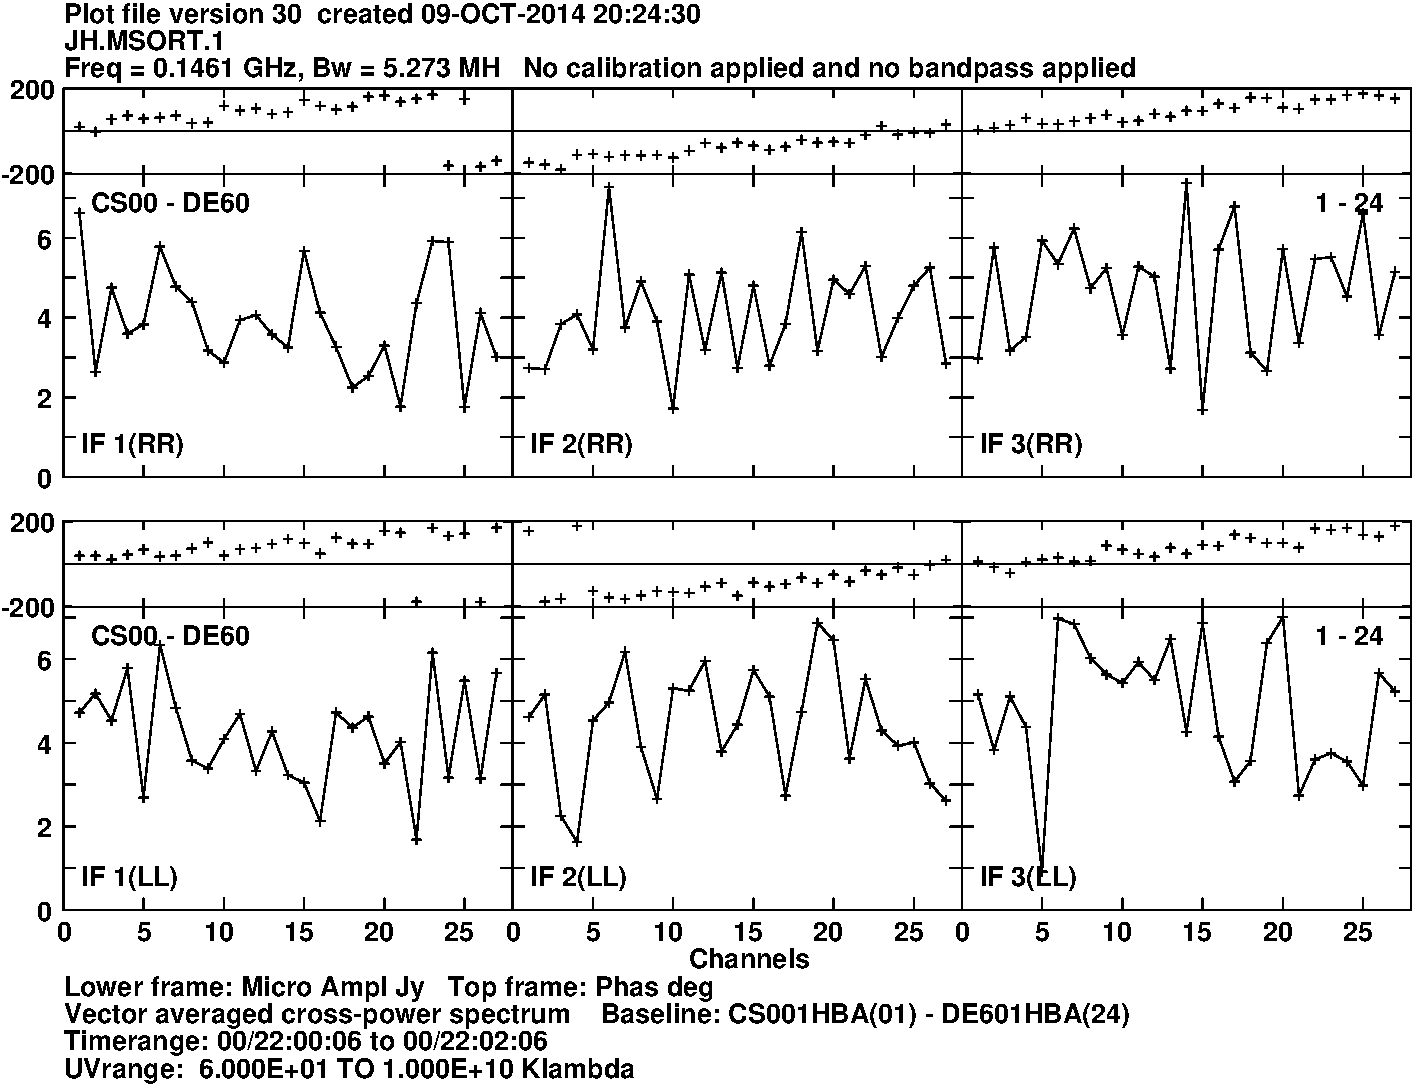
\includegraphics[width=0.7\textwidth]{figures/J0958Hprefring-crop.pdf}
    \label{fig:J0958Hprefring}
}
\subfigure[After fringe fitting]{
    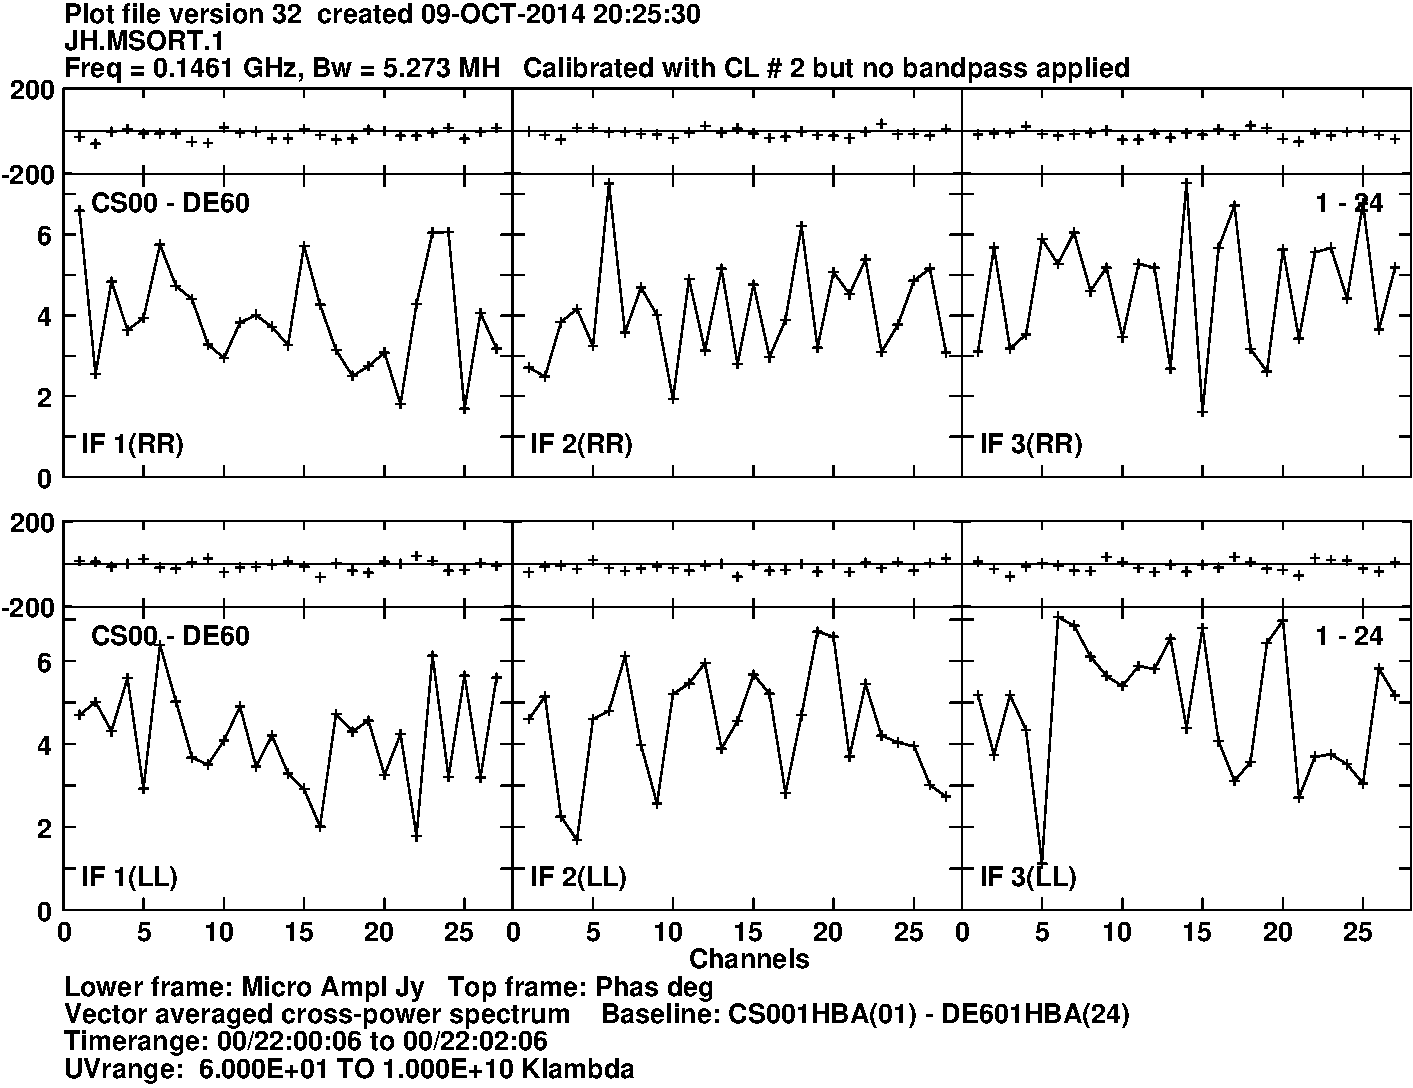
\includegraphics[width=0.7\textwidth]{figures/J0958Hpostfring-crop.pdf}
    \label{fig:J0958Hpostfring}
}
\caption{
Two figures showing the effect of fringe fitting on two minutes of data on the
baseline CS001HBA - DE601HBA for source J0958+6533 in project LC0\_26. Both
polarisations are shown, and the data are divided in three spectral windows
(IFs in AIPS) of 5.3\,MHz each.  After applying the corrections from FRING, the
phase is flat with respect to frequency, see \subref{fig:J0958Hpostfring}, as
it should be for a point source.
\label{fig:fringex}
}
\end{figure*}

Residual delays can arise due to multiple effects which are not accurately modeled in the LOFAR correlator, 
for example:

\begin{itemize}
\item Errors in station positions or target source positions
\item Instrumental effects (e.g. atomic clock drifts)
\item Propagation through the ionosphere.
\end{itemize}
If the model applied during
correlation were perfect, all stations would see a delay offset of zero for an
isolated compact source, but deviations are produced by several factors. 

Errors in station positions (and currently at a much lower level errors in the
Earth orientation parameters) produce residual delays on the order of $75$~ns,
varying with a 24~h periodicity. These errors can be expected to be greatly
reduced in the near future.  Errors in the {\em a priori} centroid position (for
example from low-frequency catalogues, with a typical error of a few arcseconds)
and/or extended structure on subarcsecond scales, introduce an additional delay.
The maximum baseline between an international station and the LOFAR core (the
correlator reference point) is 700~km (see Table~\ref{tab:baselines}); a
positional error of 1.5$^{\prime\prime}$ will lead to a residual delay of
$\sim$15 ns on this baseline.

Instabilities in the rubidium clocks used at the international stations (the
core stations share a single clock) can produce delay rates up to 20 ns per 20
min, which corresponds to about a radian per minute at 150~MHz
\citep{vanhaarlem13}.  In total, non-dispersive delays of up to $\sim100$~ns are expected.  

% and delay rates of up to $\sim$20~ns~h$^{-1}$ 

The ionospheric contribution to the delay changes as a function of time,
position, and zenith angle.  The magnitude of the changes depend on the Total
Electron Content (TEC) of the ionosphere, with a delay of $\tau_{\rm
ion}=c^{2}r_{\rm e}/(2\pi\nu^{2})\times {\rm TEC}$, being $c$ the speed of
light, $r_{\rm e}$ the classical electron radius, and $\nu$ the observed
frequency. The TEC, usually measured in TEC Units (1${\rm
TECU}=10^{16}$~electrons~m$^{-2}$), can be estimated using models derived from
observations of GPS satellites.  The models contain information on the vertical
total electron content (VTEC) during an observations. We note that the TEC
values above the stations are a lower limit of the slant ionospheric
contribution that depends on the source elevation at each station. More details
can be found in, for instance, \cite{nigl07} and \cite{sotomayor13a}.

Although the VTEC follows a 24-h trend strongly correlated with the Sun
elevation, the short-term (10--60 minute) variations between the widely
separated international stations are virtually uncorrelated.  The ionospheric
contribution typically dominates the total delay and delay rate for
international LOFAR stations. Even after a complete phase calibration, the
residual ionospheric delays between the calibrator and the target source can be
important. We have used VLBI observations (VLBA project code BD152) at 300~MHz,
or 1~m wavelength, of bright and compact pulsars at different angular
separations to obtain a rough estimate of the delay difference between sources
separated 1--5~degrees at elevations of 50--80$^{\circ}$. As a first
approximation we estimated that the dispersive delay difference between sources
at different lines of sight should be about 5~ns per degree of separation, for a
source elevation of 60$^{\circ}$.

Finally, the determination of the delays will be limited by the brightness of
the source used to calibrate them, and the sensitivity of the station. In
summary, in a normal observation the total contribution of delay to phase
changes are caused by source position and structure errors, differential
ionosphere, uncorrected instrumental delays, and noise. Delays of up to several
hundreds of ns  and delay rates of up to $\sim$20~ns~h$^{-1}$ are expected.
Table~\ref{tab:expecteddelay} summarises the main contributions and the time
scale in which they change. 

%-----------------------------------------------------------------------------
\begin{table}
\caption{Approximate delay contributions at 140~MHz to a 700~km baseline.}             % title of Table
\label{tab:expecteddelay}
\centering
\begin{tabular}{l r r}
\hline\hline
Effect  & Delay  & Time scale \\
\hline
     \multicolumn{3}{c}{Non-Dispersive}   \\
\hline
Correlator model error      & $\sim75$~ns         &  24h (periodic)   \\
Station clocks              & $\sim20$~ns        & $\sim$20~min \\
Source position offset (1.5$^{\prime\prime}$)        & $\sim15$~ns        & --  \\
\hline
     \multicolumn{3}{c}{Dispersive}   \\
\hline
Slowly varying ionosphere   & $\sim300$~ns      & $\sim$hours \\
Rapidly varying ionosphere  & $\gtrsim$10~ns         & $\sim10$~min  \\
Differential ionosphere     & 5~ns/deg sep.      & -- \\
(source elevation 60 deg)   &                    &  \\

\hline                                   %inserts single line
\end{tabular}
\end{table}
%
%-----------------------------------------------------------------------------

\subsubsection{Correcting residual delays and rates}
\label{sec:calibration}
Due to the large and time-variable delay offsets at each station, solving for
phase corrections directly (approximating the correction as constant over a
given solution time and bandwidth) would require very narrow solution intervals
for VLBI, and hence an extremely bright calibrator source ($\gtrsim10$~Jy).
However, such a source would be unlikely to be close on the sky to the target.
With a separation of perhaps tens of degrees the differential
atmosphere/ionosphere between the calibrator and the target direction would
render the derived calibration useless in the target direction. We can make use
of fainter calibrators closer to the target with the VLBI phase calibrator
known as \emph{fringe-fitting}: simultaneously solving for 3 parameters (phase,
non-dispersive delay, and phase rate) in each solution interval, allowing the
solution duration and bandwidth to be greatly extended. This technique is 
very similar to ordinary phase calibration, but in addition to solving
for phase we solve for a phase change with respect to frequency (delay) and
time (rate). 

Currently, fringe-fitting (globally) solving for delays and rates is not
available within common LOFAR software or in CASA. The current best approach is
to use the task \emph{FRING} available within the Astronomical Image Processing
System (AIPS\footnote{http://www.aips.nrao.edu/index.shtml})
\citep{greisen03a}. This task can however only solve for a \emph{linear} change
of phase with respect to frequency and time, i.e. a non-dispersive delay and
constant rate within a specific solution interval. 

Two options present themselves: to add additional parameters (covering
dispersive delay and dispersive delay rate) to the global fit, or to reduce the
solution bandwidth such that the constant dispersive delay approximation
becomes valid again.  The former option is obviously preferable from a
sensitivity perspective, but greatly expands and complicates the solution
search space.  Efforts are underway to implement such an expanded fit,
including in addition differential Faraday rotation, which becomes increasingly
important at frequencies below 100\,MHz.  First tests on individual long
baselines of LOFAR as well as baselines to other telescopes are promising, but
the algorithms are not yet sufficiently mature for public use.
Accordingly, we focus here on sources which can serve as primary calibrators
under the latter set of conditions, where solution bandwidths are limited to no
more than a few MHz and time intervals of a few minutes.

\subsubsection{What is a bright enough calibrator?}
\label{sect:brightcal}
To derive delay and rate corrections we need to find a calibrator which is
bright enough to find solutions in a small enough block in time and frequency
so that the linear approximation is valid. 
The system equivalent flux density (SEFD) of a single LOFAR core station is
approximately 1500~Jy\footnote{A LOFAR core station consists of two
sub-stations ($2\times24$ tiles) in the HBA.} at a frequency of $\sim$140~MHz
\citep{vanhaarlem13}.  An international station has twice the collecting area
of a core station at $\sim$140~MHz, so the expected SEFD is around 750 Jy.  
The theoretical 1$\sigma$ baseline sensitivity of an international
station to a (joined) HBA core station, given 3~MHz of bandwidth and 4 minutes
of observing time, is 40~mJy in a single polarisation.  
%Google: sqrt(750*1500)/(sqrt(3MHz*4*60seconds))*1000
If we require a minimum signal to noise ratio of 5 for fringe-fitting,
this means we need a calibrator brighter than 200\,mJy.

It is possible to use even weaker calibrators by forming a combined station of
all the core stations, resulting in a very sensitive station with an SEFD of
$\sim$65~Jy (see Sect. \ref{sect:ts001}).  The theoretical 1$\sigma$ baseline
sensitivity of an international station to the phased-up core station, given
3~MHz of bandwidth and 4 minutes of observing time, is hence 8~mJy in a single
polarisation.  Given this increase in sensitivity, sources with flux densities
as low as 50~mJy could in theory be used as delay/rate calibrators.  However, in
practice the sensitivity may be reduced by, for example, failing tiles,
imperfect station calibration and correlated (astronomical) noise. Also,
solution intervals shorter than 4 minutes could be required under suboptimal
ionospheric conditions. Therefore, 50\,mJy should be considered a lower limit,
in practice a flux density of more than 100\,mJy at subarcsecond scales may be
needed.

\subsubsection{What is a close enough calibrator?}
In addition to being sufficiently bright, the delay/rate calibrator must be
close enough to the target field that the differential delay between the two
fields does not lead to decorrelation when phase-only secondary calibration is
performed (as done for cm~VLBI, either using the target itself or using another
calibrator).  The solution bandwidths are narrower by a factor of $\gtrsim$10
than for cm~VLBI, which is helpful, but the ionospheric delay (inversely
proportional to observing frequency squared) is much greater, meaning that on
balance a calibrator closer than the $\lesssim$5 degrees typical for cm~VLBI
will be needed.  The maximum acceptable separation will be a strong function of
ionospheric conditions and elevation, but at face value, given a bandwidth 20
times narrower (e.g., 3 MHz vs 64 MHz) and frequency 10 times lower (140 MHz vs
1400 MHz), one would expect that the calibrator would typically need to be
separated by $\lesssim$1 degree.  This is borne out by commissioning
observations with LOFAR, which have shown acceptable results with separations
up to several degrees in favourable ionospheric conditions, and unacceptable
results with separations as small as $\sim$0.8 degrees in poor conditions.
Ideally, then, a primary calibrator for International LOFAR observations would
be located $\lesssim$1 degree from the secondary calibrator/target field to
give acceptable calibration under most circumstances. Exploration of the
distribution of compact sources at 140~MHz has shown that the density of
calibrators on the sky could be enough to overcome this restriction
\citep{moldon15}. This leads to one calibration advantage of International LOFAR
compared to cm~VLBI; since the beam of an International LOFAR station is
$\gtrsim$2 degrees across, the calibrator may easily be observed simultaneously
with the target source. Note however that care has to be taken when averaging
the data to not reduce amplitudes severely by smearing, see Sect.
\ref{sect:smearing}.  This can for example be avoided by using the
\emph{shift+averaging} procedure, see Sect. \ref{sect:shift}.


\begin{figure*}[htbp]
\begin{center}
\includegraphics[width=0.75\textwidth]{figures/J0958Hdelays-crop.pdf}
%\label{fig:J0958Hdelays}
\includegraphics[width=0.75\textwidth]{figures/J0958Hrates-crop.pdf}
%\label{fig:J0958Hrates}
\includegraphics[width=0.75\textwidth]{figures/J0958Hfringpsol-crop.pdf}
%\label{fig:J0958Hfringphases}
\caption{
Delay (top), rate (middle) and phase(bottom) corrections derived for the source
J0958+6533 at 154\,MHz by FRING for station DE601HBA for right and left
circular polarisation. These plots show the corrections derived for a 10 hour
observation (the first segment of project LC0\_026). It is clear from the rates
and phases that phases changes rapidly during the first and last hours of the
experiment. The delay solutions are more stable, although there is a large
change during the first hour. In general, the ionosphere is more stable during
midnight than at sunset or sunrise.  }

\end{center}
\end{figure*}

\subsection{Amplitude calibration of international stations}
In principle, instrumental gains within LOFAR could be tracked with time as
done in cm-VLBI (this option is currently being commissioning with the COBALT
correlator), but since this option is not yet available we rely on calibrators
with known flux density.

For core and remote stations one can use, for example, standard flux density
calibrators such as 3C196, or bright sources in low frequency catalogs such as
MSSS \citep{heald14}. However, for international stations this is in general
not possible because of the small spatial scales sampled by baselines to these
stations.  The bright standard flux calibrators, e.g. 3C196, have a very
complex structure at subarcsecond scales. If we had a good model of this
structure at our frequency of observation, we could in principle account for it
in the calibration of the international stations. Work is being done to map
well known flux density calibrators with high enough resolution, but until
these models are available we have to rely on another boot-strapping technique. 

The current best approach is to include two calibrators in the observations: a
well monitored flux density calibrator (for instance 3C196 or 3C84) and another
compact source with flux density of a few hundred mJy.  The compact calibrator
can often be the same as used to derive delay/rate solutions, see Sect,
\ref{sect:brightcal}.  While this compact source can be variable (on timescales
longer than the observation), and hence not a suitable \emph{absolute} flux density
reference, it can be used to calibrate the \emph{relative} amplitudes of all
baselines, including international stations. The absolute flux density scale can 
then be set by fitting a common scaling factor for all visibilities (including
the international baselines), by comparing the derived flux density 
for the standard flux density calibrator on short (NL) baselines, where
subarcsecond scale structure is not important.

After a phase and amplitude calibration of an International LOFAR observation,
the resulting visibilities should look similar to the ones shown in
Fig.~\ref{fig:radplot}, where we show the calibrator J0958+6533 used in
\cite{varenius15} to derive delay and rate corrections as well as the relative
amplitude scale. 

\begin{figure*}[htbp]
\begin{center}
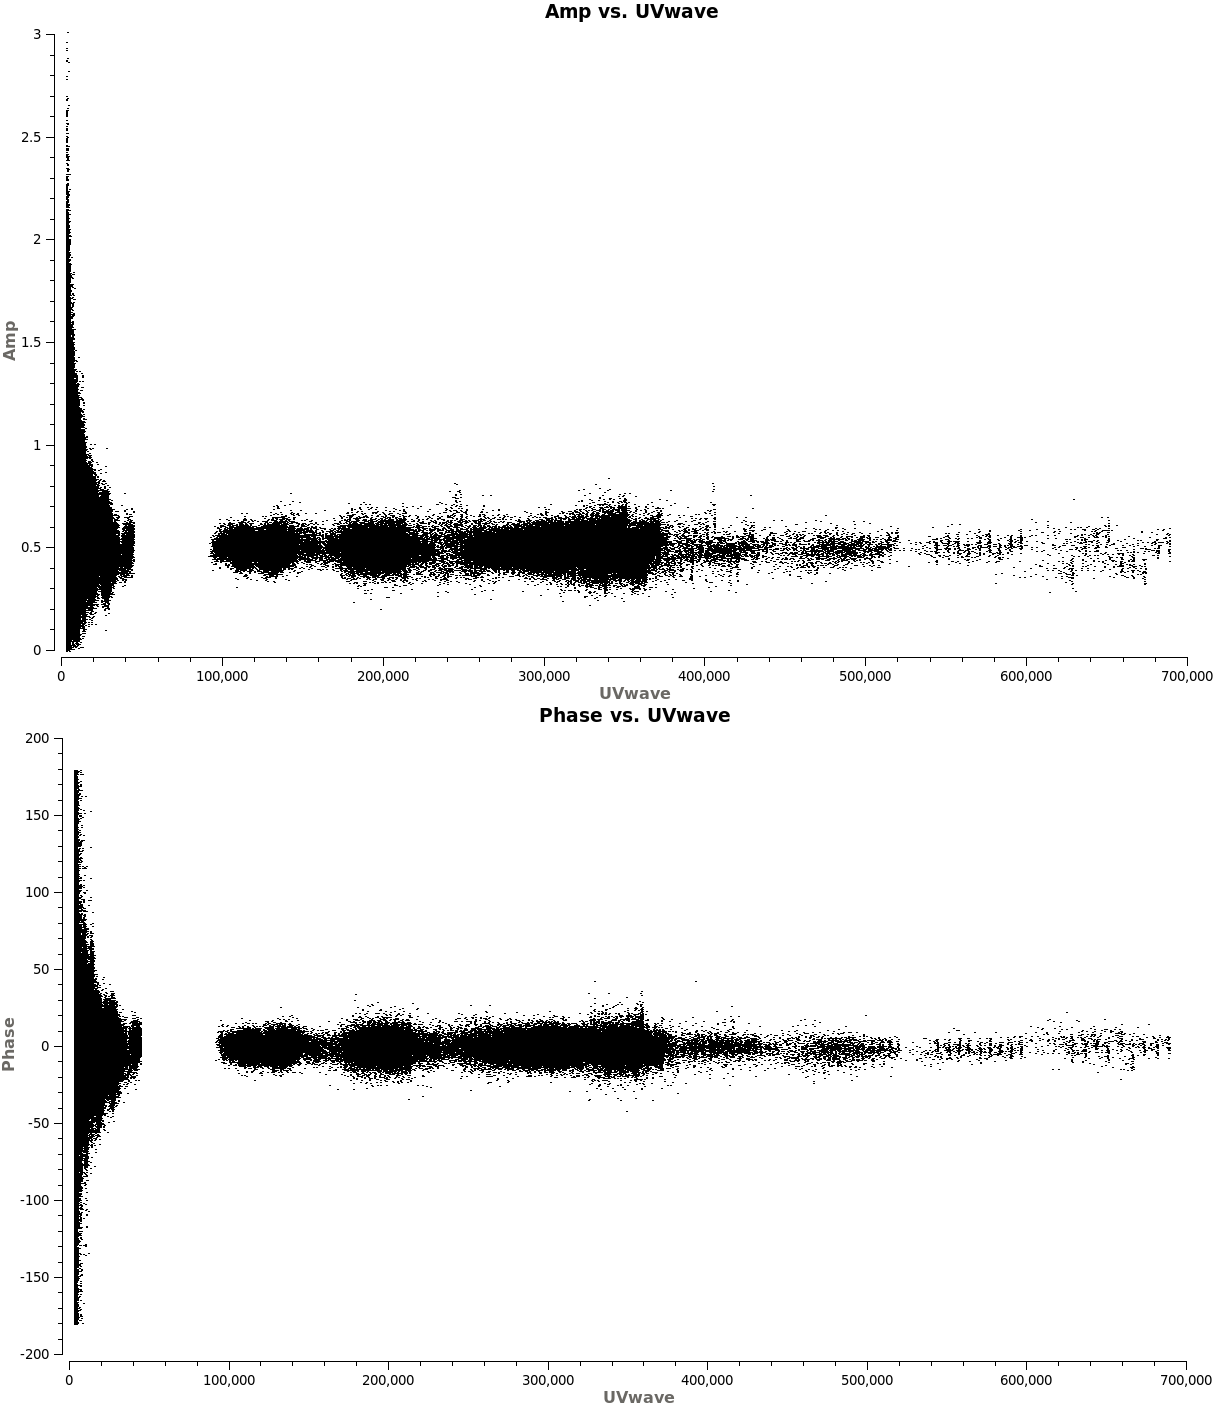
\includegraphics[width=\textwidth]{figures/radplot.png}
\caption{Amplitude (top) and phase (bottom) vs $uv$ distance for a calibrated
dataset of J0958+6533. This calibrator has a very compact component of 0.5~Jy,
mainly unresolved with the longest LOFAR baselines. We can see how the shorter
baselines are sensitive to a much more complex structure and possibly other
sources in the field.}
\label{fig:radplot}
\end{center}
\end{figure*}

\section{Observing strategy}
\label{sect:obsstrat}
For a complete International LOFAR calibration we require different calibrators
aimed to correct specific parts of the data. First, we need a very bright and
well known source with a stable flux density that is used to set the flux scale.
Although there are no good high resolution models for this kind of sources, we
can still find bright calibrators to set the flux scale of the short-baseline
part of the array, what we call the Dutch array calibrators. Some examples of
this $>30-100$~Jy can be 3C196 or 3C84, among others. The Dutch calibrator can
be considerably far away from the target field. In the future we expect to have
better high resolution models of these sources so the amplitudes of all stations
could be corrected with the same calibrator. Second, we need compact and
moderately bright (above 100--200~mJy) source at a separation of about 1 degree
or less. This source, the primary calibrator, can be used to solve for
non-dispersive delays of blocks of $\sim3$~MHz data. Finally, after application
of the solutions from the primary calibrator it is common to use a secondary
calibrator\footnote{A secondary calibrator is often referred to as an
``in-beam'' calibrator in VLBI if it is close enough to the target source to be
observed contemporaneously} closer to the target source. This second phase-only
calibration is used to refine the calibration errors that result from the
spatial (and temporal) interpolation of the primary solutions.  Ideally, the
secondary calibrator should be at $\sim$arcmin separations from the target
source.  Because solving for phases is a problem with fewer degrees of freedom
than fringe fitting, lower S/N data can be used.  Additionally, because the bulk
delay has already been removed the residual delays should be small and even more
bandwidth can be combined in a single solution for a further improvement in S/N.
A secondary calibrator can therefore be considerably fainter (usually
$\gtrsim$5~mJy). If bright enough, the target source can be used to derive this
correction.  This typical calibration strategy is illustrated in
Figure~\ref{fig:calstrategy}. In comparison with a typical cm-VLBI strategy a
LOFAR observation can be more efficient because the size of the LOFAR station
beam (see Table~\ref{tab:res}) is large enough that the primary and the
secondary calibrators are observed simultaneously.

\begin{figure*}[] %figure1
\center 
%\resizebox{1.0\hsize}{!}{
\includegraphics[width=\textwidth]{figures/vlbi_sketch.pdf}
%}
\caption{Typical calibration setup for cm VLBI (left) and International LOFAR
(right).  Note that in some cases the target may itself function as the
secondary calibrator.  A secondary calibrator is not always required for cm
VLBI, but will almost always be needed for International LOFAR, unless the
primary calibrator is fortuitously close.  The larger field of view of LOFAR
means that both the primary and secondary calibrators will always be observed
contemporaneously, unlike in cm VLBI, where nodding between the primary 
calibrator and target is typically required (shown by the double arrow in the
left panel).}
\label{fig:calstrategy}
\end{figure*}


When preparing an International LOFAR observation one should take into account
the different calibrators needed, considering that primary and secondary
compact calibrators are currently unknown. Probably a small part of the
observation should be aimed to identify calibrators. \cite{moldon15} proposed
the following approach for an International LOFAR observation: 

\begin{enumerate}
\item Identify candidate primary calibrators up to separations of a few degrees 
    by using any of the criteria discussed in Sect.~5.3 in
    \cite{moldon15};
\item Conduct a short observation in snapshot mode as described
in Sect.~\ref{findcalib} before the science observation to identify
the best primary calibrator (or calibrators).
\item If required and time permits, follow up with a ``full bandwidth'' snapshot observation to 
identify one or more secondary calibrators;
\item Set up the scientific observation to dwell on the field 
containing the primary calibrator and the target/secondary calibrator;
\item Include periodic scans (every $\sim$ hour) on a bright Dutch array 
calibrator to calibrate the core stations in order to form the tied station.
\item Shift phase centre to primary calibrator, preprocess and obtain delay solutions 
as described in this paper, apply them to the unshifted dataset;
\item If a secondary calibrator is to be used and is not yet identified, select 10 minutes
of data and perform shift/averaging to candidate secondary calibrator sources;
\item If secondary calibrator is used: shift and average primary-calibrated dataset, 
image and selfcalibrate, apply solutions to the unshifted dataset;
\item Shift and average calibrated dataset, image and (if needed) selfcalibrate target.
\end{enumerate}

In the near future, the pipeline used for this project will be developed, in
collaboration with the LOFAR operations team, into an expanded form capable of
carrying out the approach described above.  This pipeline will be made available
to all International LOFAR observers, delivering a reduced data volume for
long-baseline observations and enabling calibrated data to be more quickly
produced.


\section{Practical considerations}
\label{sect:practical}

The calibration of International LOFAR data is not fundamentally different from
any other radio interferometric data, although special care should be taken
regarding, for example, the phase calibration using VLBI techniques. However,
there are some particular practical considerations that could help the observer
to reduce this type of data. A detailed description of the steps and software
that can be used to reduce these data can be found in The LOFAR Imaging
Cookbook\footnote{\url{http://www.astron.nl/radio-observatory/lofar/lofar-imaging-cookbook}}.
In this section we list some hints and useful procedures that are needed when
planning and reducing International LOFAR data.


\subsection{Optimising use of available bandwidth}\label{sec:bandwidth}
It is possible to distribute LOFAR bandwidth over a number of beams to
simultaneously observe different regions of the sky. In particular, it is
possible to divide the bandwidth on target(s) and calibrator, which provides a
continuous source calibration without the need of regularly nodding from target
to calibrator. Another possibility is to distribute the bandwidth among a large
number of sources to search for suitable calibrators. For example one can
generate 30 beams to observe simultaneously 30 sources with 3~MHz bandwith as a
fast way to search for suitable compact calibrators for an
International LOFAR observation \citep[see i.e.][]{moldon15}. 

\subsubsection{Unequal distribution of subbands on target and
calibrators}\label{sec:bwdist} 
If your calibrator is bright, you can use fewer subbands on the calibrator, and
thereby get better sensitivity on the target. To use fringe finding, we need to
sample accurately the residual delay/rate slope (and possibly curvature at low
frequencies) present in the data. This can be done with sparse sampling in
frequency, where the optimal coverage is achieved by spreading the subbands as
a powerlaw density with denser placement of subbands at lower frequencies
\citep{marti-vidal10}. The advantage of this approach is that more bandwidth
can be placed on the target.  The disadvantage is that the calibration becomes
a bit more demanding. One reason for this is that the UVFITS format used by
AIPS (for running fringe fitting) requires data in all channels.  If we do not
have contiguous subband coverage in frequency, we need to insert fake data and
flag that (e.g. using NDPPP) before reading the data into AIPS.  This will
cause an increase in data volume which will slow down processing.  Also,
spreading the subbands sparsely is always a risk in case your calibrator is
weaker than you think. A detailed discussion can be found in
\cite{marti-vidal10}, where the authors analyse how to distribute subbands
specifically for LOFAR observations for optimal fringe detection.

\subsubsection{The shift + averaging procedure}\label{sect:shift}
Given the high resolution obtained with the
International LOFAR observations, imaging of the region restricted by the time
and frequency average of the data (see Table~\ref{tab:res}) would require a
very high computational cost. If one is interested in multiple objects within
the station beam, one can phase-shift (and re-project) the $uv$-data to each
object before averaging.  After correlation, the full-resolution visibility
dataset can be shifted and averaged multiple times, to the positions of all the
target sources and possibly to one or more nearby calibrators. Starting in
cycle four, it will be possible to request shifting and averaging of data to
multiple phase centres within a beam as a part of a normal observation.

\subsection{Finding calibrators}\label{findcalib}

Until a good catalogue of compact sources at MHz frequencies is available, it is
important to take into account that a science observation might require a
preparatory search of calibrators. A fast method using the distribution of
bandwidth between many sources (see Sect.~\ref{sec:bwdist}) is described in
\cite{moldon15}. A pre-selection based on a number of parameters from existing
catalogues, such as the low-frequency spectral index, and the flux, can be
performed to optimize the search. In particular the most useful catalogues are
the VLSS, at 74~MHz, 4~m wavelength \citep{lane12a}, the WENSS catalogue at
325~MHz, 92 cm wavelength \citep{rengelink97}, and specially The Multifrequency
Snapshot Sky Survey (MSSS), which comes from LOFAR observations \citep{heald14}.
Also, compact calibrators at mas scales detected with cm-VLBI are probably also
compact at LOFAR frequencies. Although there is a strong correlation, a cm-VLBI
calibrator may not be suitable for LOFAR in case it is variable or if it has
inverted or gigahertz peaked spectra. An updated list of cm-VLBI calibrators
covering the whole sky can be found in \url{http://astrogeo.org/rfc/}.

\cite{moldon15} showed that there is a density of $\sim1$ good calibrator per
square degree based on two fields with Galactic latitudes of $+26.6^{\circ}$ and
$+43.4^{\circ} $. However, we expect less compact sources at lower Galactic
latitudes due to interstellar scattering. The Galactic electron density model
NE2001 \citep{cordes02} predicts an scattering at a galactic latitude of
$50^{\circ}$ of almost 100~mas at 150~MHz, which is five times smaller than our
resolution. However, the scattering is about 300~mas, similar to our beamsize,
at latitudes of 5--10$^{\circ}$, depending on the longitude. Therefore,
observations below a Galactic latitude of 10$^{\circ}$ are likely to be affected
by scattering on the longest baselines, and the effect should be severe below
about 2$^{\circ}$, especially towards the Galactic Center. 

\subsection{Form a combined station}
\label{sect:ts001}
When studying very compact structures, the shortest baselines do not add
much interesting information while they slow down the calibration process.
The core stations can be added to form a coherent ``tied station'' (TS001) that
keeps the total core sensitivity on the long baselines to the international
stations.  Since the core stations are under similar atmospheric conditions and
they share the same clock only slow changes in their amplitudes and phases are
expected, and thus they can be calibrated by observing a bright primary
calibrator once every $\sim1$~hr. TS001 can be formed by summing baseline
visibilities with the NDPPP task ``StationAdder''.  After this step, all
original visibilities with core-core baselines can be discarded using the NDPPP
task ``Filter'' to significantly reduce the data volume.

One important benefit of having a tied station is that it works as a very
sensitive station. This tied-array station aids in the derivation of calibration
solutions to the international stations with FRING, and can be used as a
reference station. We note that a tied-station formed by adding the whole core
has a very small (5\% amplitude loss at 30$''$ distance from phase centre) field
of view. Although this is rarely a problem for deriving FRING solutions, care is
needed if using such combined data to image extended objects.

%In Fig.~\ref{fig:CSvsTS} we show calibrated amplitudes and phases for some
%baselines from some remote stations to a single core station and to the tied
%station formed by coherently combining 23 core stations.

%\begin{figure}
%%\sidecaption[t]
%\begin{center}
%\includegraphics[width=\textwidth]{figures/amp_uv_CSRS_TSRS.png}
%\caption{Amplitude (top) and phase (top) as a function of uv-distance for the
%baselines between CS001 (left) and TS001 (right) to four remote stations.}
%\label{fig:CSvsTS}
%\end{center}
%\end{figure}

\subsection{Getting LOFAR data into AIPS}
The task FRING in AIPS can be used to remove residual delays and rates in the
data. However, AIPS requires that the data are in circular polarisation (LOFAR
usually stores data in linear polarisation). AIPS also requires the
data to be converted from measurement set (MS) to the UVFITS file format.
In this section we describe how this can be achieved. 

\subsubsection{Converting linear to circular polarisation}

Differential Faraday rotation introduces rapid phase changes with frequency
into linear polarisation data on long baselines. For long-baseline observations
is preferable to work in a circular (R,L) polarisation basis. In this basis,
the ionospheric disturbances are transformed from coupled amplitude/phase
effects (as in the linear X,Y basis) to phase only effects. Since differential
Faraday rotation does not mix R and L polarisations we may calibrate RR and LL
independently. Furthermore, standard VLBI techniques like fringe fitting work
in a circular (R,L) polarisation basis. To run FRING in AIPS, the data have to be
converted to circular polarisation.

There are two common ways to convert LOFAR measurement sets to circular polarisation:
either using BBS and Table Query Language (TAQL), which uses the BBS beam model,
or using the custom software \emph{mscorpol} developed by T. D. Carozzi, which uses
its own beam model. Detailed instructions on how to use these tools are provided in the LOFAR Imaging cookbook.

\subsubsection{Converting measurement set to UVFITS}
Since AIPS understands the UVFITS-format, but not Measurement Sets (MS)
we need to convert the data from MS to UVFITS. This can be done using e.g.
the tool \emph{ms2uvfits} available at the LOFAR cluster or the task \emph{exportuvfits} in CASA.
Note that it is important to have contigous data in frequency (e.g. by filling 
missing subbands with fake data) and to have data present for all baselines (i.e.
by flagging instead of partially filtering antennas). 



\begin{acknowledgement}
This chapter and all the techniques and procedures described in it are based on
the work and many useful contributions of the LOFAR long baselines working
group. AIPS is produced and maintained by the National Radio Astronomy
Observatory, a facility of the National Science Foundation operated under
cooperative agreement by Associated Universities, Inc.

\end{acknowledgement}

%\input{references01}

\bibliographystyle{aa}
\bibliography{chapter13}

\end{document}
